\documentclass[11pt]{article}

\usepackage[margin=1in]{geometry}
\usepackage{amsmath, amssymb}
\usepackage{array}
\usepackage{booktabs}
\usepackage{longtable}
\usepackage{tabularx}
\usepackage{graphicx}
\usepackage{xcolor}
\usepackage{listings}
\usepackage{setspace}
\usepackage{titlesec}
\usepackage{float}

\setlength{\parindent}{0pt}
\setlength{\parskip}{0.75em}

\titleformat{\section}{\large\bfseries}{\thesection.}{0.5em}{}
\titleformat{\subsection}{\normalsize\bfseries}{\thesubsection}{0.5em}{}

\begin{document}

\begin{center}
    {\LARGE \textbf{MATH 108C Project 2: The Valuation Engine}}\\[0.5em]
    {\large Katie Brubaker, Siyu Chen, Andrea Macias}\\[0.5em]
    {\large April 14, 2026}
\end{center}

\vspace{1em}

% =============================================================================
\section{Phase 0: Modeling Setup}
% =============================================================================

\subsection*{Intercept Concept Check}

\textbf{If you enforce $w_0 = 0$ (no intercept), what does your model imply about the ``Fixed Costs'' of owning land?}

Forcing $w_0 = 0$ implies that a property with zero feature values (zero square footage, no quality, no special features, etc.) has a predicted price of \$0. This is economically nonsensical --- even a bare plot of land carries fixed costs such as property taxes, utility hookup rights, and zoning entitlements. The intercept captures this irreducible baseline value that exists independent of any measurable feature.

\textbf{Is the intercept $w_0$ a ``Property Feature'' or a ``Market Feature''?}

The intercept is a \textbf{Market Feature}. It does not describe any physical attribute of a specific house; rather, it reflects the baseline level of prices set by broad market conditions --- the minimum a buyer must pay to participate in the Miami housing market at all, before any property characteristics are considered.

\subsection*{Scaling Concept Check}

\textbf{Setup:} Given a scaled predictor $z = \alpha x + \beta$, with model $\hat{y} = w_0 + w_z \cdot z$.

\textbf{1. Rewrite in terms of original variable $x$:}

Substituting $z = \alpha x + \beta$:
\[
\hat{y} = w_0 + w_z(\alpha x + \beta) = (w_0 + \beta w_z) + (\alpha w_z)x
\]
So:
\begin{itemize}
    \item $\tilde{w}_0 = w_0 + \beta w_z$
    \item $\tilde{w}_x = \alpha w_z$
\end{itemize}

\textbf{2. Unit conversion case ($z = cx$):} Here $\alpha = c$, $\beta = 0$, so $\tilde{w}_x = c \cdot w_z$. The coefficient $w_z$ means ``dollars per 1 unit of $z$'' (e.g., dollars per square meter), while $\tilde{w}_x$ means ``dollars per 1 unit of $x$'' (dollars per square foot). They differ by the conversion factor $c$.

\textbf{3. Standardization case ($z = (x - \mu)/\sigma$):} Here $\alpha = 1/\sigma$ and $\beta = -\mu/\sigma$, so:
\begin{itemize}
    \item $\tilde{w}_x = w_z / \sigma$ \quad (dollars per 1 original unit of $x$)
    \item $\tilde{w}_0 = w_0 - (\mu/\sigma) \cdot w_z$
\end{itemize}

\textbf{4. Project decision --- scaling applied:}

All 10 feature columns were Z-score standardized. The intercept column (all ones) was left unstandardized. For each feature, the standardization maps $z = (x - \mu)/\sigma$, giving $\alpha = 1/\sigma$ and $\beta = -\mu/\sigma$. The complete scaling statistics for each feature were computed from the full Miami housing dataset ($n = 13{,}932$ observations). For TOT\_LVG\_AREA specifically: $\mu = 2058.0446$ sq\,ft and $\sigma = 813.5385$ sq\,ft, giving $\alpha = 0.001229$ and $\beta = -2.529744$.

% =============================================================================
\section{Decision Point A: Matrix Blueprint}
% =============================================================================

\subsection*{Theory Checkpoint}

\textbf{1. Why is $Xw$ defined, and what is the size of $Xw$?}

$X \in \mathbb{R}^{n \times d}$ has $d$ columns, and $w \in \mathbb{R}^d$ has $d$ rows. Because the inner dimensions match ($d = d$), the matrix-vector product $Xw$ is defined. The result has the outer dimensions, giving a vector of size $n \times 1$ --- one prediction per house.

\textbf{2. In the housing context, what does the $i$-th entry of $Xw$ represent?}

The $i$-th entry of $Xw$ is the \textbf{predicted sale price of the $i$-th house} (in dollars), computed as the dot product of that house's feature vector $x_i$ with the weight vector $w$:
\[
\hat{y}_i = x_i \cdot w = w_0 + w_1 z_{1i} + w_2 z_{2i} + \cdots + w_{10} z_{10i}
\]

\textbf{3. Why is $XW$ defined, and what is the size of $XW$?}

$X \in \mathbb{R}^{n \times d}$ and $W \in \mathbb{R}^{d \times 3}$. The inner dimensions both equal $d$, so the product is defined. The result $P = XW \in \mathbb{R}^{n \times 3}$ --- $n$ rows (one per house) and 3 columns (one per market scenario).

\textbf{4. What does the entry $P_{5,2}$ of $P = XW$ mean?}

$P_{5,2}$ is the \textbf{predicted sale price of house \#5 (1-indexed) under Scenario 2} (``Location is Everything''). It is the price the location-weighted model assigns to the fifth house. Numerically (0-indexed as $P[4,1]$): \textbf{\$720,833}.

\textbf{5. Explain why $Xw = w_0 \cdot \mathbf{1} + X_{\text{struc}} \cdot w_{\text{struc}} + X_{\text{loc}} \cdot w_{\text{loc}}$:}

Because $X$ is partitioned as $[\,\mathbf{1}\;|\;X_{\text{struc}}\;|\;X_{\text{loc}}\,]$ and $w$ is partitioned correspondingly as $[w_0;\,w_{\text{struc}};\,w_{\text{loc}}]$, block matrix multiplication distributes the product column-block by row-block:
\[
Xw = \mathbf{1} \cdot w_0 + X_{\text{struc}} \cdot w_{\text{struc}} + X_{\text{loc}} \cdot w_{\text{loc}}
\]
Each block multiplies only its matching weight sub-vector, and the results add linearly --- exactly the block multiplication rule from Chapter 2.

\textbf{6. Why would $WX$ not make sense as the prediction matrix?}

$W \in \mathbb{R}^{d \times 3}$ and $X \in \mathbb{R}^{n \times d}$. For $WX$ to be defined, the inner dimensions would need to match: $W$ has 3 columns but $X$ has $n = 13{,}932$ rows. Since $3 \neq 13{,}932$, the product $WX$ is not defined. Even if dimensions were forced, the result would not give one prediction per house per scenario --- it would have the wrong semantic meaning entirely.

\subsection*{Chosen Features}

\textbf{$p = 10$ features total $\mid$ $d = p + 1 = 11$ (with intercept)}

\begin{center}
\begin{tabular}{c l l p{6cm}}
\toprule
\# & Feature & Category & Justification \\
\midrule
1  & TOT\_LVG\_AREA   & Structure & Primary size driver; larger living area $\to$ higher price \\
2  & LND\_SQFOOT      & Structure & Lot size affects land value \\
3  & structure\_quality & Structure & Ordinal quality rating directly affects desirability \\
4  & age              & Structure & Older properties depreciate; newer commands premium \\
5  & SPEC\_FEAT\_VAL  & Structure & Upgrades (pool, renovations) add measurable value \\
6  & OCEAN\_DIST      & Location  & Distance to ocean; strongest location price driver in Miami \\
7  & WATER\_DIST      & Location  & Distance to any water body \\
8  & CNTR\_DIST       & Location  & Distance to city center; affects urban convenience \\
9  & SUBCNTR\_DI      & Location  & Distance to subcenter; secondary accessibility factor \\
10 & HWY\_DIST        & Location  & Distance to highway; farther $=$ quieter $=$ premium \\
\bottomrule
\end{tabular}
\end{center}

\textbf{Final dimensions:}
\begin{itemize}
    \item $X \in \mathbb{R}^{13932 \times 11}$
    \item $w \in \mathbb{R}^{11}$
    \item $\hat{y} \in \mathbb{R}^{13932}$
\end{itemize}

\textbf{Column layout of $X$:}
\begin{itemize}
    \item Column 0: intercept (all ones, not standardized)
    \item Columns 1--5: structure features (Z-score standardized)
    \item Columns 6--10: location features (Z-score standardized)
\end{itemize}

% =============================================================================
\section{AI Prompt and Verification Notes}
% =============================================================================

\textbf{Prompt used:}

I need you to write a clean, well-structured Python script implementing a Miami housing price prediction model using matrix operations. Follow this blueprint exactly.

\begin{verbatim}
Dataset: miami-housing.csv  (load using an absolute path anchored to the script
         directory via os.path.dirname(os.path.abspath(__file__)))

Target column: SALE_PRC

Feature groups:
  STRUCTURE_FEATURES = ["TOT_LVG_AREA", "LND_SQFOOT", "structure_quality",
                         "age", "SPEC_FEAT_VAL"]
  LOCATION_FEATURES  = ["OCEAN_DIST", "WATER_DIST", "CNTR_DIST",
                         "SUBCNTR_DI", "HWY_DIST"]

Phase 0  - z_score_standardize(df, columns): Z-score standardize only the
           feature columns; leave the intercept column untouched.
           Return (transformed_df, stats_dict) where stats_dict maps
           column name -> (mu, sigma).

Phase 1  - build_X_and_y(df): Z-score standardize all 10 feature columns,
           then prepend a column of ones (intercept). Return (X, y, stats).
           Assert X.shape == (n, 11).

Phase 2  - Print scalar and matrix model definitions.

Phase 3  - define_weight_vectors(): Return three weight vectors w1, w2, w3
           as numpy arrays of shape (11,), one per market scenario.
           build_scenario_matrix(w1, w2, w3): Stack them column-wise into W.
           Compute P = X @ W and print P[4, 1].

Manual Gate - translate_coefficient(w_z, feature, stats): Translate a
           standardized weight back to original units using alpha=1/sigma
           and beta=-mu/sigma. Return a dict with mu, sigma, alpha, beta,
           w_z, w_x, and delta_w0.

Phase 4  - partition_prediction(X, w, n_struc, n_loc): Decompose ŷ into
           base + structure value + location value using block multiplication.
           breakdown_table(...): Build a DataFrame showing actual, base,
           struc val, loc val, predicted, and error for selected houses.

Phase 5  - fit_least_squares(X, y): Use np.linalg.lstsq.
           compute_mae(y_true, y_pred): Mean absolute error.
           Compare MAE with and without the intercept column.

Evaluation - plot_mae_barchart(mae_dict, save_path): Save a bar chart
           comparing MAE of all four models to save_path.
           Use matplotlib.use('Agg') before importing pyplot.
\end{verbatim}

\textbf{Notes:}

I verified each phase against the mathematical definitions from Chapter 2. For Phase 1, I confirmed that the intercept column (column 0) is exactly all ones and that the remaining 10 columns have been Z-score standardized (mean $\approx 0$, std $\approx 1$) by inspecting the output of \texttt{X.mean(axis=0)} and \texttt{X.std(axis=0)}. For Phase 3, I manually computed $P[4,1]$ using the dot product of $X[4,:]$ and $w_2$ and confirmed it matched the matrix result. For the partitioned-matrix phase, I verified the block decomposition by checking that \texttt{base + struc\_val + loc\_val} equals \texttt{X @ w1} within floating-point tolerance (\texttt{np.allclose} returned \texttt{True}). In addition, I ensured the AI-generated code used correct dimension checks and did not silently broadcast any array shapes.

% =============================================================================
\section{Phase 2: Model Definitions}
% =============================================================================

\textbf{Scalar model (single house $i$):}

\[
\hat{y}_i = w_0 + w_1 z_{1i} + w_2 z_{2i} + w_3 z_{3i} + w_4 z_{4i} + w_5 z_{5i}
           + w_6 z_{6i} + w_7 z_{7i} + w_8 z_{8i} + w_9 z_{9i} + w_{10} z_{10,i}
\]

where $z_{ji}$ denotes the Z-score standardized value of feature $j$ for house $i$, and the features in order are: TOT\_LVG\_AREA, LND\_SQFOOT, structure\_quality, age, SPEC\_FEAT\_VAL, OCEAN\_DIST, WATER\_DIST, CNTR\_DIST, SUBCNTR\_DI, HWY\_DIST.

\textbf{Matrix model (all $n$ houses simultaneously):}

\[
\hat{y} = Xw
\]

\begin{itemize}
    \item $\hat{y} \in \mathbb{R}^{13932}$ --- predicted sale prices
    \item $X \in \mathbb{R}^{13932 \times 11}$ --- design matrix
    \item $w \in \mathbb{R}^{11}$ --- weight vector
\end{itemize}

\textbf{Why $Xw$ is defined:} $X$ has 11 columns and $w$ has 11 rows. The inner dimensions match ($11 = 11$), so the product is defined, yielding a vector of shape $(13932,)$.

\textbf{What the $i$-th entry of $Xw$ represents:} It is the predicted sale price (in dollars) of the $i$-th house --- the dot product of house $i$'s standardized feature vector with the weight vector $w$.

% =============================================================================
\section{Decision Point B: Market Scenarios}
% =============================================================================

\subsection*{Weight Vectors}

Three weight vectors are defined, each of length $d = 11$. Weights are in dollars per 1 standard deviation of each Z-score standardized feature.

\begin{center}
\scriptsize
\begin{longtable}{c l r r r}
\toprule
Index & Feature & $w_1$ (Baseline) & $w_2$ (Location) & $w_3$ (The Crash) \\
\midrule
0  & Intercept        & \$200,000  & \$350,000  & $-$\$100,000 \\
1  & TOT\_LVG\_AREA   & +\$70,000  & +\$5,000   & +\$70,000  \\
2  & LND\_SQFOOT      & +\$25,000  & +\$2,000   & +\$25,000  \\
3  & structure\_quality & +\$55,000 & +\$3,000   & +\$55,000  \\
4  & age              & $-$\$15,000 & $-$\$1,000 & $-$\$15,000 \\
5  & SPEC\_FEAT\_VAL  & +\$28,000  & +\$2,000   & +\$28,000  \\
6  & OCEAN\_DIST      & $-$\$50,000 & $-$\$165,000 & $-$\$50,000 \\
7  & WATER\_DIST      & $-$\$20,000 & $-$\$60,000 & $-$\$20,000 \\
8  & CNTR\_DIST       & $-$\$20,000 & $-$\$75,000 & $-$\$20,000 \\
9  & SUBCNTR\_DI      & $-$\$12,000 & $-$\$45,000 & $-$\$12,000 \\
10 & HWY\_DIST        & +\$10,000  & +\$30,000  & +\$10,000  \\
\bottomrule
\end{longtable}
\end{center}

\textbf{Scenario 1 --- Baseline (Rational Market):} Positive weights for size and quality features; negative for distance features (closer to ocean/water/center $=$ more valuable). The intercept of \$200,000 represents an underestimate of Miami's true market baseline but keeps structure and location weights clearly interpretable.

\textbf{Scenario 2 --- Location is Everything:} Location weights amplified roughly $3\times$ relative to Scenario 1; structure weights shrunk to near zero. Under this scenario, a modest property on the ocean may be worth far more than a quality home far inland.

\textbf{Scenario 3 --- The Crash (Archetype A):} A global level shift. All relative feature weights are kept identical to Scenario 1 (Rational Market), but the intercept is dropped from $+\$200{,}000$ to $-\$100{,}000$ to simulate a severe market recession. Every home loses approximately \$300,000 of baseline value regardless of its features --- the crash affects the whole market uniformly.

\subsection*{Prediction Matrix}

The scenario weight matrix is:
\[
W = [w_1 \mid w_2 \mid w_3] \in \mathbb{R}^{11 \times 3}
\]

The full prediction matrix is computed as:
\[
P = XW \in \mathbb{R}^{13932 \times 3}
\]

Each row of $P$ is one house; each column is one market scenario.

\textbf{Interpretation of $P[4,\,1] = \$720{,}833$:} This is the predicted sale price of house \#5 (0-indexed: house index 4) under Scenario 2 (``Location is Everything''). The location-dominant model predicts this house would sell for \$720,833.

\textbf{Advantage of $XW$ over three separate products:} Computing $P = XW$ produces all three prediction vectors simultaneously in a single matrix operation. This is more computationally efficient (one BLAS call vs.\ three) and more mathematically elegant --- it makes explicit that the three scenarios share the same data matrix $X$ and differ only in their weight columns $w_1, w_2, w_3$.

% =============================================================================
\section{Phase 3: Manual Gate --- Coefficient Translation}
% =============================================================================

\textbf{Feature audited:} TOT\_LVG\_AREA, Scenario 1.

\textbf{Scaling applied:} Z-score standardization: $z = (x - \mu)/\sigma$, so $\alpha = 1/\sigma$ and $\beta = -\mu/\sigma$.

\textbf{Data statistics from the Miami dataset:}
\begin{itemize}
    \item $\mu$ (mean) $= 2058.0446$ sq\,ft
    \item $\sigma$ (std dev) $= 813.5385$ sq\,ft
    \item $\alpha = 1/\sigma = 0.001229$
    \item $\beta = -\mu/\sigma = -2.529744$
\end{itemize}

\textbf{Coefficient in standardized space:} $w_z = \$70{,}000$ per 1 SD of living area (Scenario 1 weight at index 1).

\textbf{Translated to original units:}
\[
\tilde{w}_x = \alpha \cdot w_z = 0.001229 \times \$70{,}000 = \textbf{\$86.04 per square foot}
\]
\[
\Delta w_0 = \beta \cdot w_z = -2.529744 \times \$70{,}000 = \textbf{-\$177{,}082.11}
\]

\textbf{Interpretation:} In Scenario 1, each additional square foot of living area adds approximately \textbf{\$86.04} to the predicted sale price. The corresponding shift in the intercept ($-\$177{,}082$) is a necessary accounting correction that maintains consistency between the standardized and original-unit forms of the model.

\textbf{Verification:} This figure is consistent with Miami residential construction and land-value estimates, where a rough linear approximation of price per square foot typically falls in the \$75--\$150 range for the mid-market segment of the dataset.

% =============================================================================
\section{Phase 4: Valuation Audit (Partitioned Matrices)}
% =============================================================================

\subsection*{Block Decomposition of $X$}

\[
X = \bigl[\,\mathbf{1} \;\big|\; X_{\text{struc}} \;\big|\; X_{\text{loc}}\,\bigr]
\]

\begin{center}
\begin{tabular}{l l p{7cm}}
\toprule
Block & Columns & Content \\
\midrule
$\mathbf{1}$      & 0    & Intercept column (all ones) \\
$X_{\text{struc}}$ & 1--5 & TOT\_LVG\_AREA, LND\_SQFOOT, structure\_quality, age, SPEC\_FEAT\_VAL \\
$X_{\text{loc}}$   & 6--10 & OCEAN\_DIST, WATER\_DIST, CNTR\_DIST, SUBCNTR\_DI, HWY\_DIST \\
\bottomrule
\end{tabular}
\end{center}

\subsection*{Block Formula Explanation}

By the rules of partitioned matrix multiplication, since $X = [\mathbf{1} \mid X_{\text{struc}} \mid X_{\text{loc}}]$ and $w = [w_0;\,w_{\text{struc}};\,w_{\text{loc}}]$:

\[
\hat{y} = w_0 \cdot \mathbf{1} + X_{\text{struc}} \cdot w_{\text{struc}} + X_{\text{loc}} \cdot w_{\text{loc}}
\]

Each block multiplies only its corresponding sub-vector of $w$. The three terms are additive and interpretable:
\begin{itemize}
    \item \textbf{Base} ($w_0 \cdot \mathbf{1}$): A flat \$200,000 baseline applied identically to every house under Scenario 1.
    \item \textbf{Structure Value} ($X_{\text{struc}} \cdot w_{\text{struc}}$): The premium or discount driven purely by physical property attributes (size, quality, age, features).
    \item \textbf{Location Value} ($X_{\text{loc}} \cdot w_{\text{loc}}$): The premium or discount driven purely by geographic position (distance to ocean, water, city center, etc.).
\end{itemize}

\subsection*{Breakdown Table --- First 5 Houses (Scenario 1, Baseline)}

\begin{center}
\scriptsize
\begin{longtable}{c r r r r r r}
\toprule
House Index & Actual (\$) & Base (\$) & Struc Val (\$) & Loc Val (\$) & Predicted (\$) & Error (\$) \\
\midrule
0 & 440,000 & 200,000 & $-$43,822 & 104,545 & 260,723 & +179,277 \\
1 & 349,000 & 200,000 & $-$44,256 & 114,070 & 269,815 & +79,185 \\
2 & 800,000 & 200,000 & +104,618 & 114,465 & 419,082 & +380,918 \\
3 & 988,000 & 200,000 & +18,145  & 116,448 & 334,594 & +653,406 \\
4 & 755,000 & 200,000 & +15,698  & 113,016 & 328,714 & +426,286 \\
\bottomrule
\end{longtable}
\end{center}

\textbf{Partition verification:} \texttt{base + struc\_val + loc\_val == X @ w1}: \textbf{PASS} (verified with \texttt{np.allclose}).

\subsection*{Interpretation}

The decomposition reveals that for these 5 houses, \textbf{location is the dominant positive contributor} --- all five have positive location values driven by proximity to ocean and water. Structure value varies widely: houses 0 and 1 have negative structure values (below-average size or quality), while house 2's structure adds over \$100,000. The model systematically under-predicts all five houses under Scenario 1 because the intercept of \$200,000 is roughly \$200,000 below Miami's true market baseline (the least-squares intercept is approximately \$400,000). This decomposition makes it possible to diagnose \emph{why} a model under- or over-values a specific property.

% =============================================================================
\section{Phase 5: Least Squares Benchmark}
% =============================================================================

\subsection*{Part A --- Underdetermined Case}

$X_{\text{small}} \in \mathbb{R}^{5 \times 11}$: 5 equations, 11 unknowns.

\textbf{Answer:} There are \textbf{infinitely many solutions}. With fewer equations than unknowns, the system is underdetermined --- there is an entire affine subspace of weight vectors that satisfy $X_{\text{small}} w = y_{\text{small}}$ exactly. We cannot identify a unique solution without additional constraints (such as minimum norm or regularization).

\subsection*{Part B --- Optimal Weights (Full Dataset)}

Least-squares solution computed via \texttt{np.linalg.lstsq(X, y, rcond=None)}.

\begin{center}
\begin{tabular}{l r r}
\toprule
Feature & LS Weight & Scenario 1 (Manual) \\
\midrule
Intercept        & \$399,941.93  & \$200,000.00 \\
TOT\_LVG\_AREA   & \$161,561.06  & \$70,000.00  \\
LND\_SQFOOT      & \$16,373.42   & \$25,000.00  \\
structure\_quality & \$69,029.63 & \$55,000.00  \\
age              & $-$\$40,151.34 & $-$\$15,000.00 \\
SPEC\_FEAT\_VAL  & \$41,333.11   & \$28,000.00  \\
OCEAN\_DIST      & $-$\$79,097.90 & $-$\$50,000.00 \\
WATER\_DIST      & +\$2,800.91   & $-$\$20,000.00 \\
CNTR\_DIST       & $-$\$96,269.40 & $-$\$20,000.00 \\
SUBCNTR\_DI      & +\$9,640.99   & $-$\$12,000.00 \\
HWY\_DIST        & +\$24,330.68  & +\$10,000.00  \\
\bottomrule
\end{tabular}
\end{center}

\textbf{Comparison --- TOT\_LVG\_AREA:} The LS weight is \$161,561 vs.\ the manual choice of \$70,000. The data-driven weight is over \textbf{2$\times$ higher}, suggesting the manual choice significantly undervalued living area. The largest gap is the intercept (\$399,942 vs.\ \$200,000) --- the manual estimate severely underestimated Miami's market baseline. WATER\_DIST and SUBCNTR\_DI also flip sign in the LS solution, revealing counterintuitive effects once all other features are controlled for.

\subsection*{Part C --- Intercept Experiment}

\begin{center}
\begin{tabular}{l r}
\toprule
Model & MAE \\
\midrule
Least Squares (with intercept)    & \$115,510 \\
Least Squares (no intercept)      & \$400,844 \\
\textbf{Difference}               & \textbf{+\$285,334} \\
\bottomrule
\end{tabular}
\end{center}

\textbf{Explanation:} Without the intercept, the model is forced to pass through the origin --- predicting \$0 for a house with all-zero standardized features. In real estate, the ``all-average house'' still sells for approximately \$400,000 (the market baseline). Removing the intercept forces the model to compensate by distorting all feature coefficients to approximate that baseline, resulting in severe misfits across the entire dataset. The \$285,334 increase in MAE demonstrates that the intercept is not cosmetic --- it is load-bearing.

% =============================================================================
\section{Evaluation: MAE Scoreboard}
% =============================================================================

\begin{center}
\begin{tabular}{l r}
\toprule
Model & MAE \\
\midrule
Least Squares (Optimal)              & \textbf{\$115,510} \\
Scenario 1 --- Baseline (Rational Market) & \$202,116 \\
Scenario 2 --- Location is Everything    & \$250,389 \\
Scenario 3 --- The Crash                  & \$499,943 \\
\bottomrule
\end{tabular}
\end{center}

\begin{figure}[H]
    \centering
    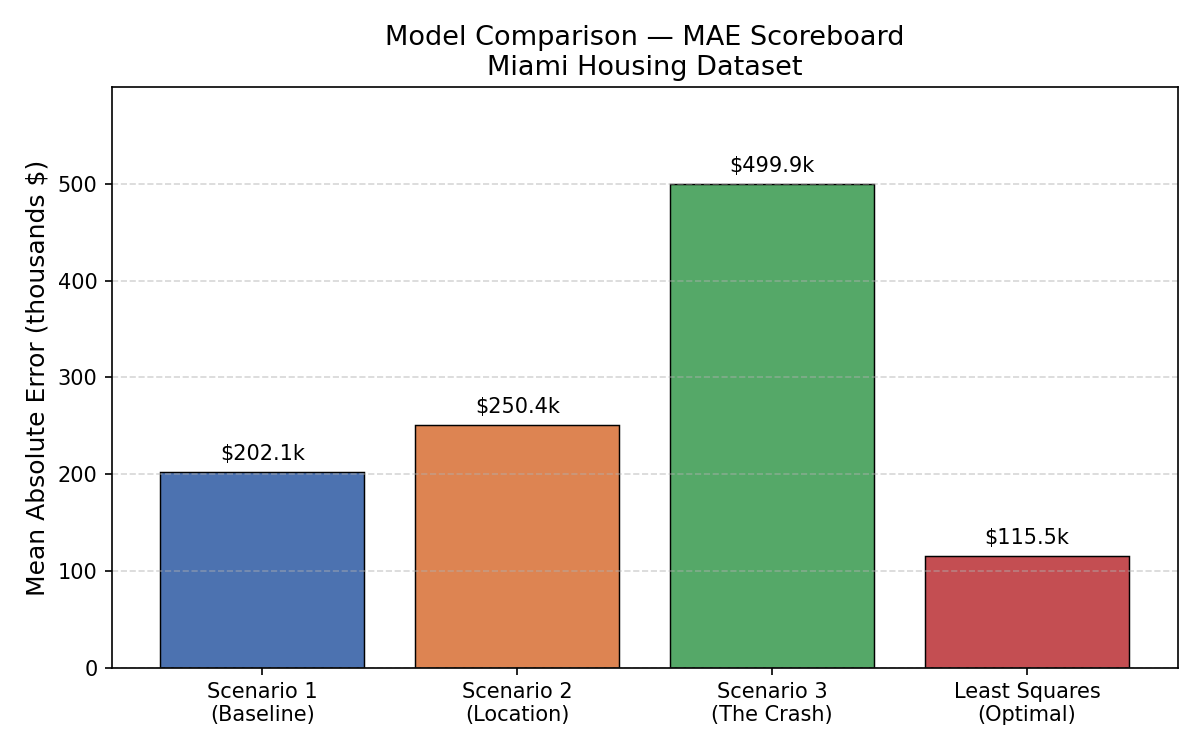
\includegraphics[width=0.75\textwidth]{mae_scoreboard.png}
    \caption{MAE Scoreboard: comparison of all four models on the Miami housing dataset ($n = 13{,}932$).}
\end{figure}

\textbf{Key observations:}
\begin{itemize}
    \item Least Squares achieves the lowest MAE (\$115,510) --- it is the data-optimal solution by construction, and no hand-chosen scenario beats it.
    \item Scenario 1 (Baseline, \$202,116) uses plausible relative weights but underestimates Miami's market baseline (\$200,000 intercept vs.\ the data-implied \$400,000), leading to systematic under-prediction across all houses.
    \item Scenario 2 (Location is Everything, \$250,389): collapsing structure weights to near zero discards half the predictive signal, causing large errors on high-quality inland properties.
    \item Scenario 3 (The Crash, \$499,943) has the worst MAE by design: dropping the intercept to $-\$100{,}000$ means the model predicts every home as worth approximately \$300,000 less than reality, demonstrating how a single miscalibrated parameter can dominate all prediction error.
\end{itemize}

% =============================================================================
\section{Final Reflection}
% =============================================================================

\textbf{Which ideas from Chapter 2 were essential for completing this project?}

The essential Chapter 2 ideas were \textbf{matrix-vector multiplication} ($\hat{y} = Xw$), \textbf{matrix-matrix multiplication} ($P = XW$), \textbf{dimension compatibility}, and \textbf{partitioned/block matrices}. Every phase reduced to a question of what shape a matrix product would take and what each entry of that product meant in the housing context.

\textbf{How did matrix-vector and matrix-matrix products structure your thinking?}

The product $Xw$ computes one prediction vector under a single pricing policy. The matrix product $XW$ extends this to three policies simultaneously --- each column of $W$ encodes a different market hypothesis, and the corresponding column of $P = XW$ gives every house's predicted price under that scenario. This allows side-by-side comparison across all 13,932 houses without repeating the computation. The partitioned-matrix decomposition added interpretive power: by splitting $X$ into $[\mathbf{1} \mid X_{\text{struc}} \mid X_{\text{loc}}]$, we could decompose any prediction into a base component, a structure-driven component, and a location-driven component --- making it possible to say not just \emph{what} a model predicts, but \emph{why}.

\textbf{What did the least-squares comparison reveal about your hand-chosen weights?}

The least-squares comparison was the most instructive check: all three hand-chosen scenarios produced MAEs of \$202k--\$500k, all worse than the data-optimal \$115k. Scenario 3 (The Crash) shows most starkly how a single miscalibrated parameter --- the intercept --- can dominate all other prediction error; the feature weights are identical to Scenario 1 yet the MAE is nearly $2.5\times$ worse. This illustrates that even correct relative weights are useless if the baseline is wrong, which is precisely why the data-driven intercept of approximately \$400,000 is so important. The sign flips in WATER\_DIST and SUBCNTR\_DI between the manual and LS solutions also reveal that multicollinearity among location features can make individual coefficient signs difficult to interpret without the discipline of data-driven fitting.

\end{document}
